\section{Experiment}

\frame{\frametitle{Index}\tableofcontents[currentsection,subsectionstyle=show/show/shaded]}

\begin{frame}
	\frametitle{Environmental Setup}

	\begin{block}{SeARCH Group Hex}
		\begin{description}
			\item [] Intel\textsuperscript{\textregistered} Xeon\textsuperscript{\textregistered} X5650
			\item [2] processors per node;
			\item [6] cores per processor;
			\item [-] Intel\textsuperscript{\textregistered} HyperThreading Technology;
			\item [2.66] GHz clock frequency;
			\item [12 to 48] GB of RAM;
			\item [Tesla C2070]
			\begin{description}
				\item [1] Tesla CPU;
				\item [448] CUDA cores;
				\item [1.15] GHz clock frequency;
				\item [515] Gflops peak (double);
				\item [6] GB dedicated memory;
				\item [144] GB/sec memory bandwidth;
			\end{description}
		\end{description}
	\end{block}
\end{frame}

\begin{frame}{Methodology}
	\begin{itemize}
		\vfill
		\item Limited execution: 5000 iterations;
		\vfill
		\item Median of 10 executions;
		\vfill
		\item 62 MB test case;
		\vfill
		\item Measurements focused on final speedups;
		\vfill
	\end{itemize}
\end{frame}

\begin{frame}
	\frametitle{Speedups}
	\begin{figure}
		\centering
		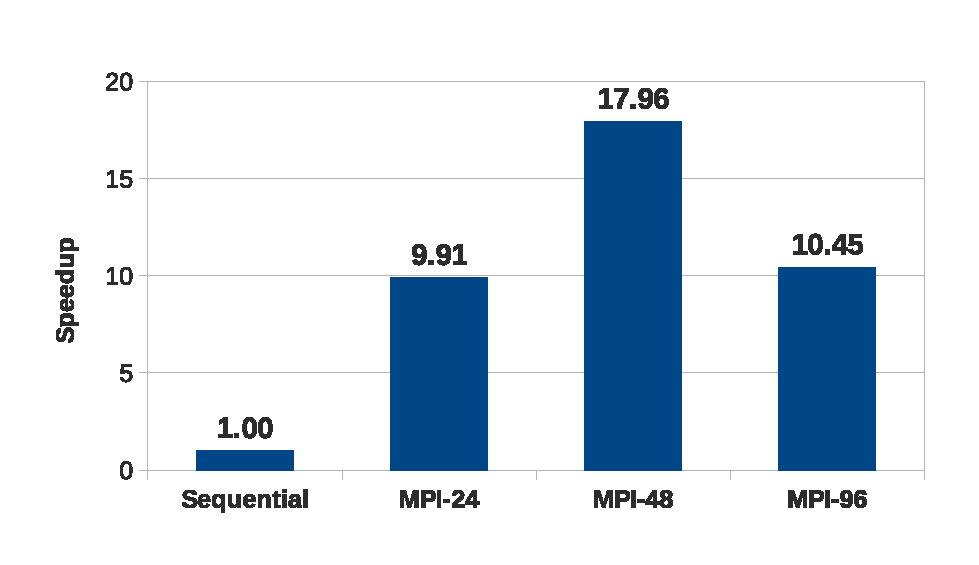
\includegraphics[width=0.8\textwidth]{graph_comparison_all.eps}
	\end{figure}
\end{frame}
